\chapter{Grænseflader}
Dette afsnit beskriver systemets grænseflader og forklare hvordan bruger interagere med systemet.

\section{Brugergrænseflade}
Brugergrænsefladen består af en webapplikation, hvor bruger kan lave nye flyveopsætninger, gemme flyveopsætninger og overvåge drone status. 

\section{Webapplikation}
På figur \ref{fig:mockup_login} ses login vinduet, som bruger bliver præsenteret for når der ønskes at interagere med systemet. Her vil bruger kunne logge ind og lave flyveopsætninger, se gamle flyveruter og billeder fra tidligere flyvninger. Der accepteres kun tre fejlindtastninger til login. Hvis de tre forsøg overskrides, bliver bruger låst og administrator skal kontaktes.

\vspace{-5pt}
%Login mockup
\begin{figure}[H]
	\centering
	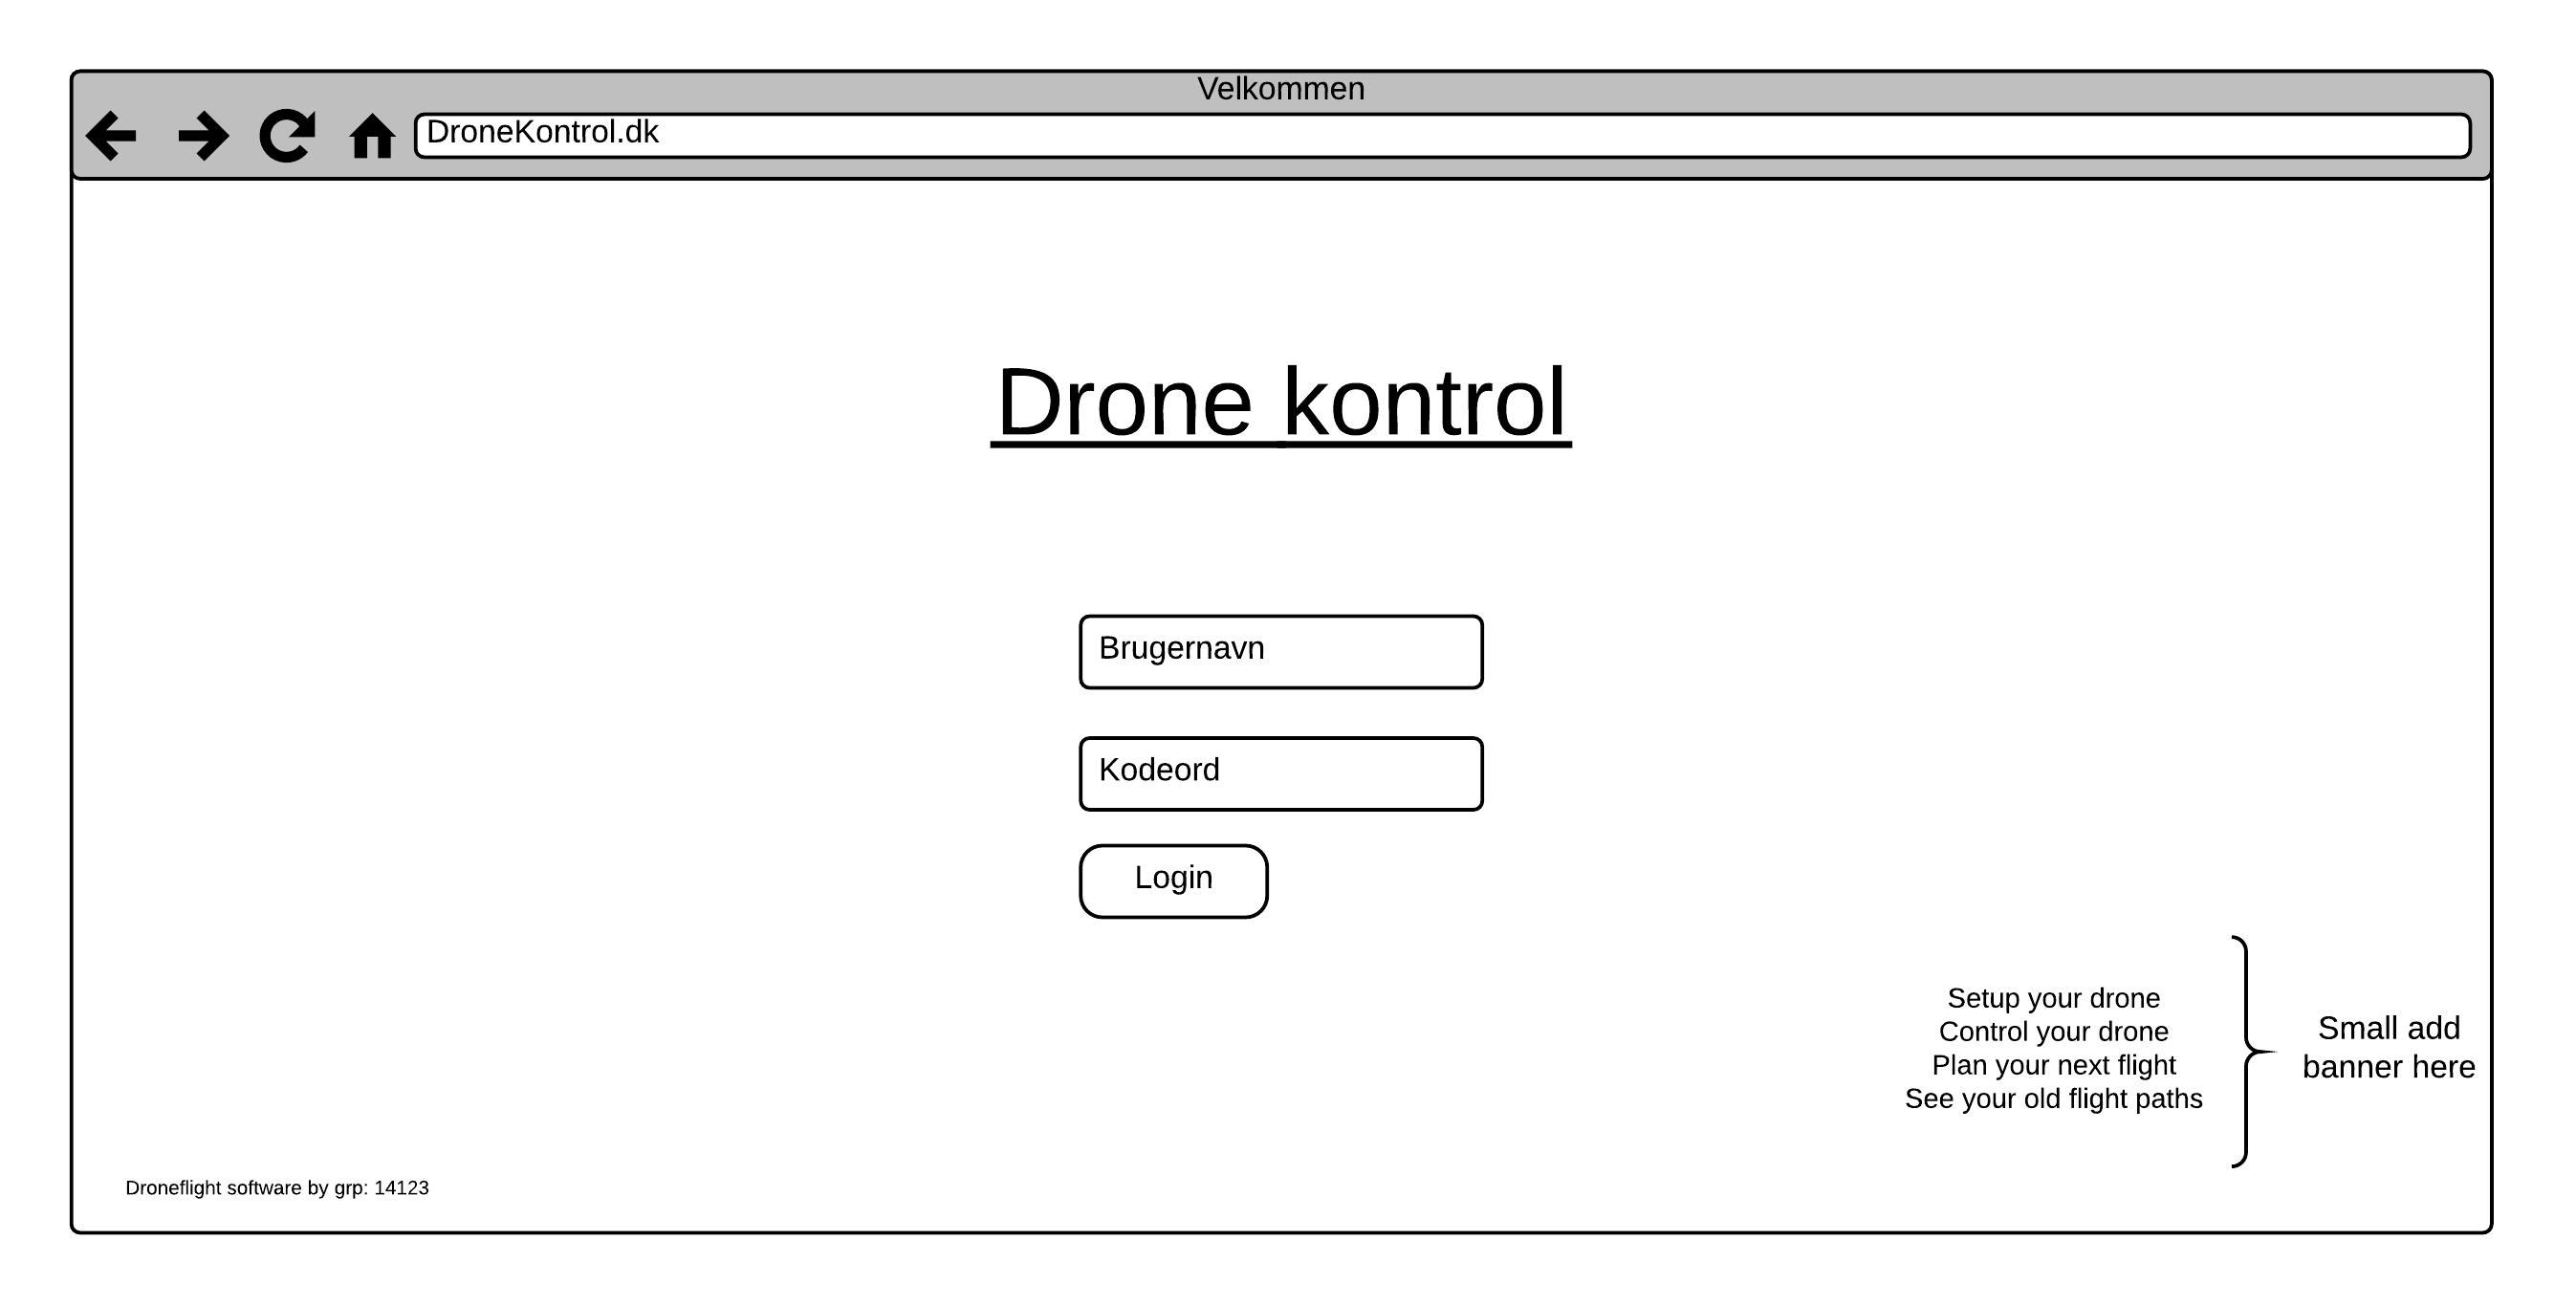
\includegraphics[width=0.9\textwidth]{Billeder/UI_mockups/login.png}
	\vspace{-.5cm}
	\caption{Login vindue}
	\label{fig:mockup_login}
\end{figure}

 \newpage

Efter login præsenteres bruger for webapplikationens forside, se figur \ref{fig:mockup_welcome}. 
Fra forsiden kan bruger se om dronen er online, tilgå Flight bootcamp, som er en quick-guide til flyveopsætning og se en liste med information af de sidste flyvninger. Øverst på siden kan bruger tilgå opsætning af ny flyvning og den fulde liste med tidligere flyvninger.

\vspace{-5pt}
 %Index mockup
 \begin{figure}[H]
 	\centering
 	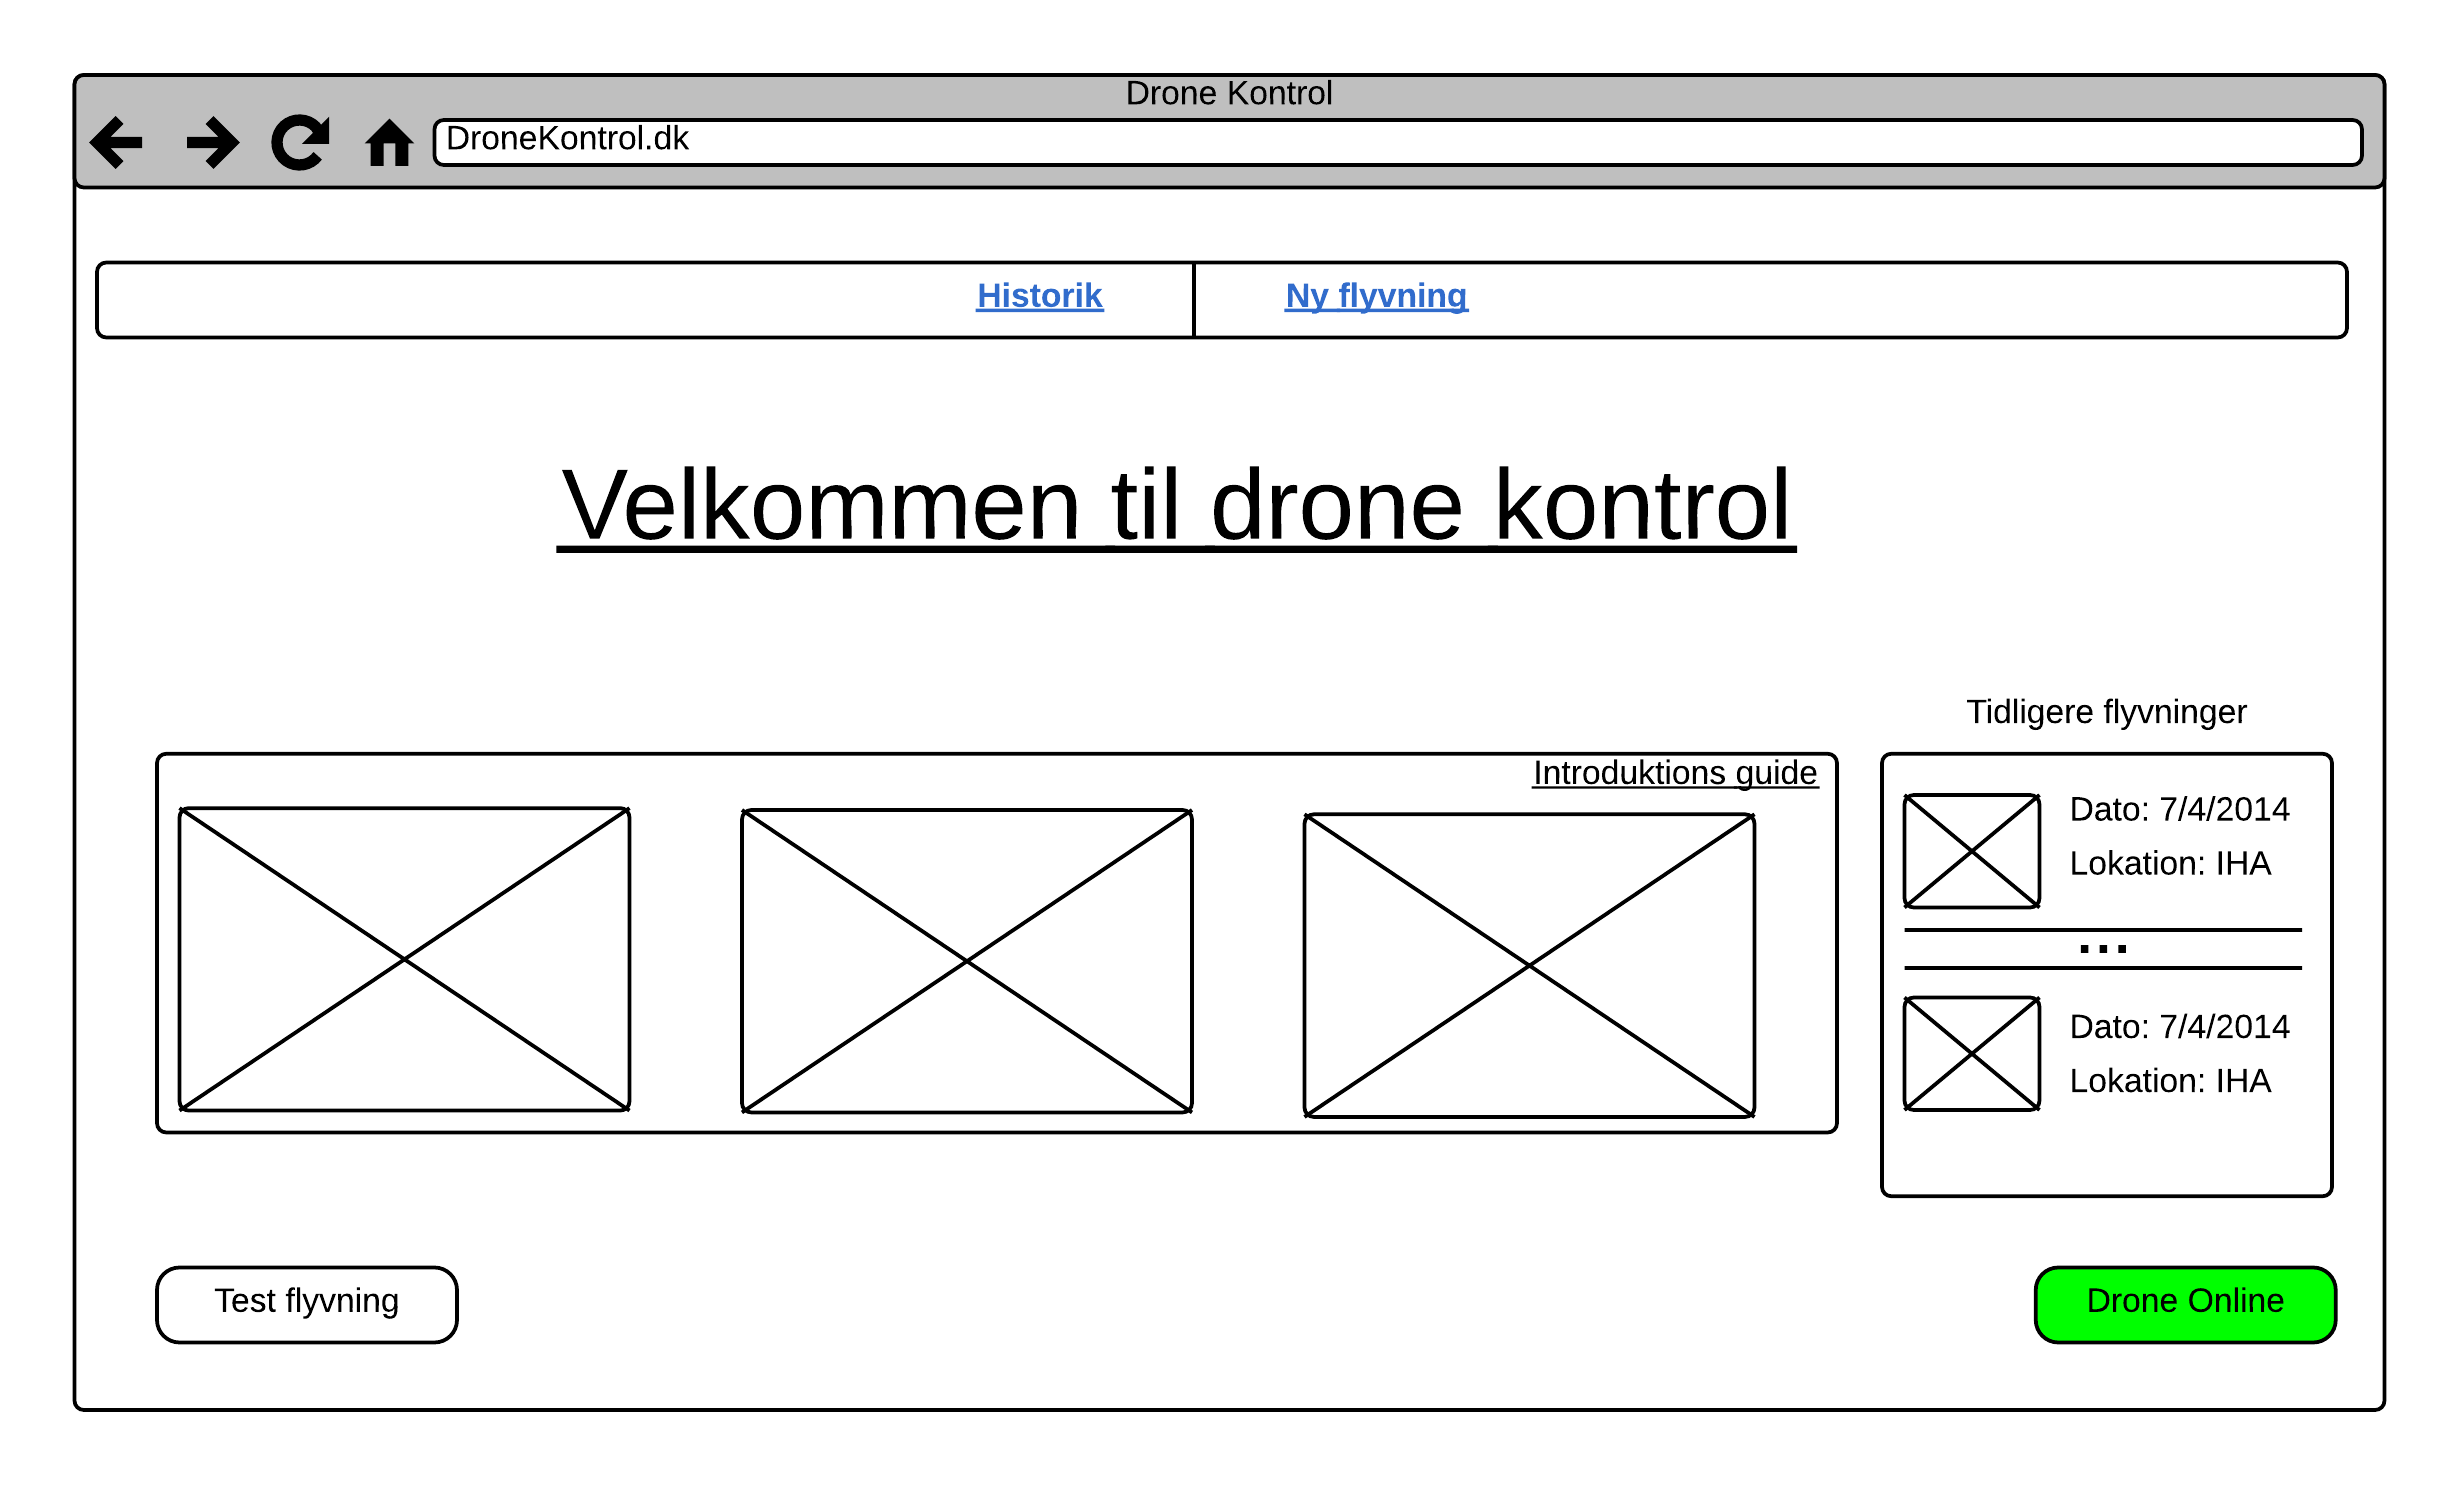
\includegraphics[width=0.9\textwidth]{Billeder/UI_mockups/index.png}
 	\vspace{-.5cm}
 	\caption{Velkommen vindue}
 	\label{fig:mockup_welcome}
 \end{figure} 

I historik menuen har bruger mulighed for at se alle tidligere flyvninger. De tidligere flyvninger præsenteres med hver sin mappe, og mapperne er struktureret efter dato. Mappestrukturen gør det nemt og hurtigt at finde data ønskede flyvninger.

\vspace{-5pt}
%Archive mockup
\begin{figure}[H]
	\centering
	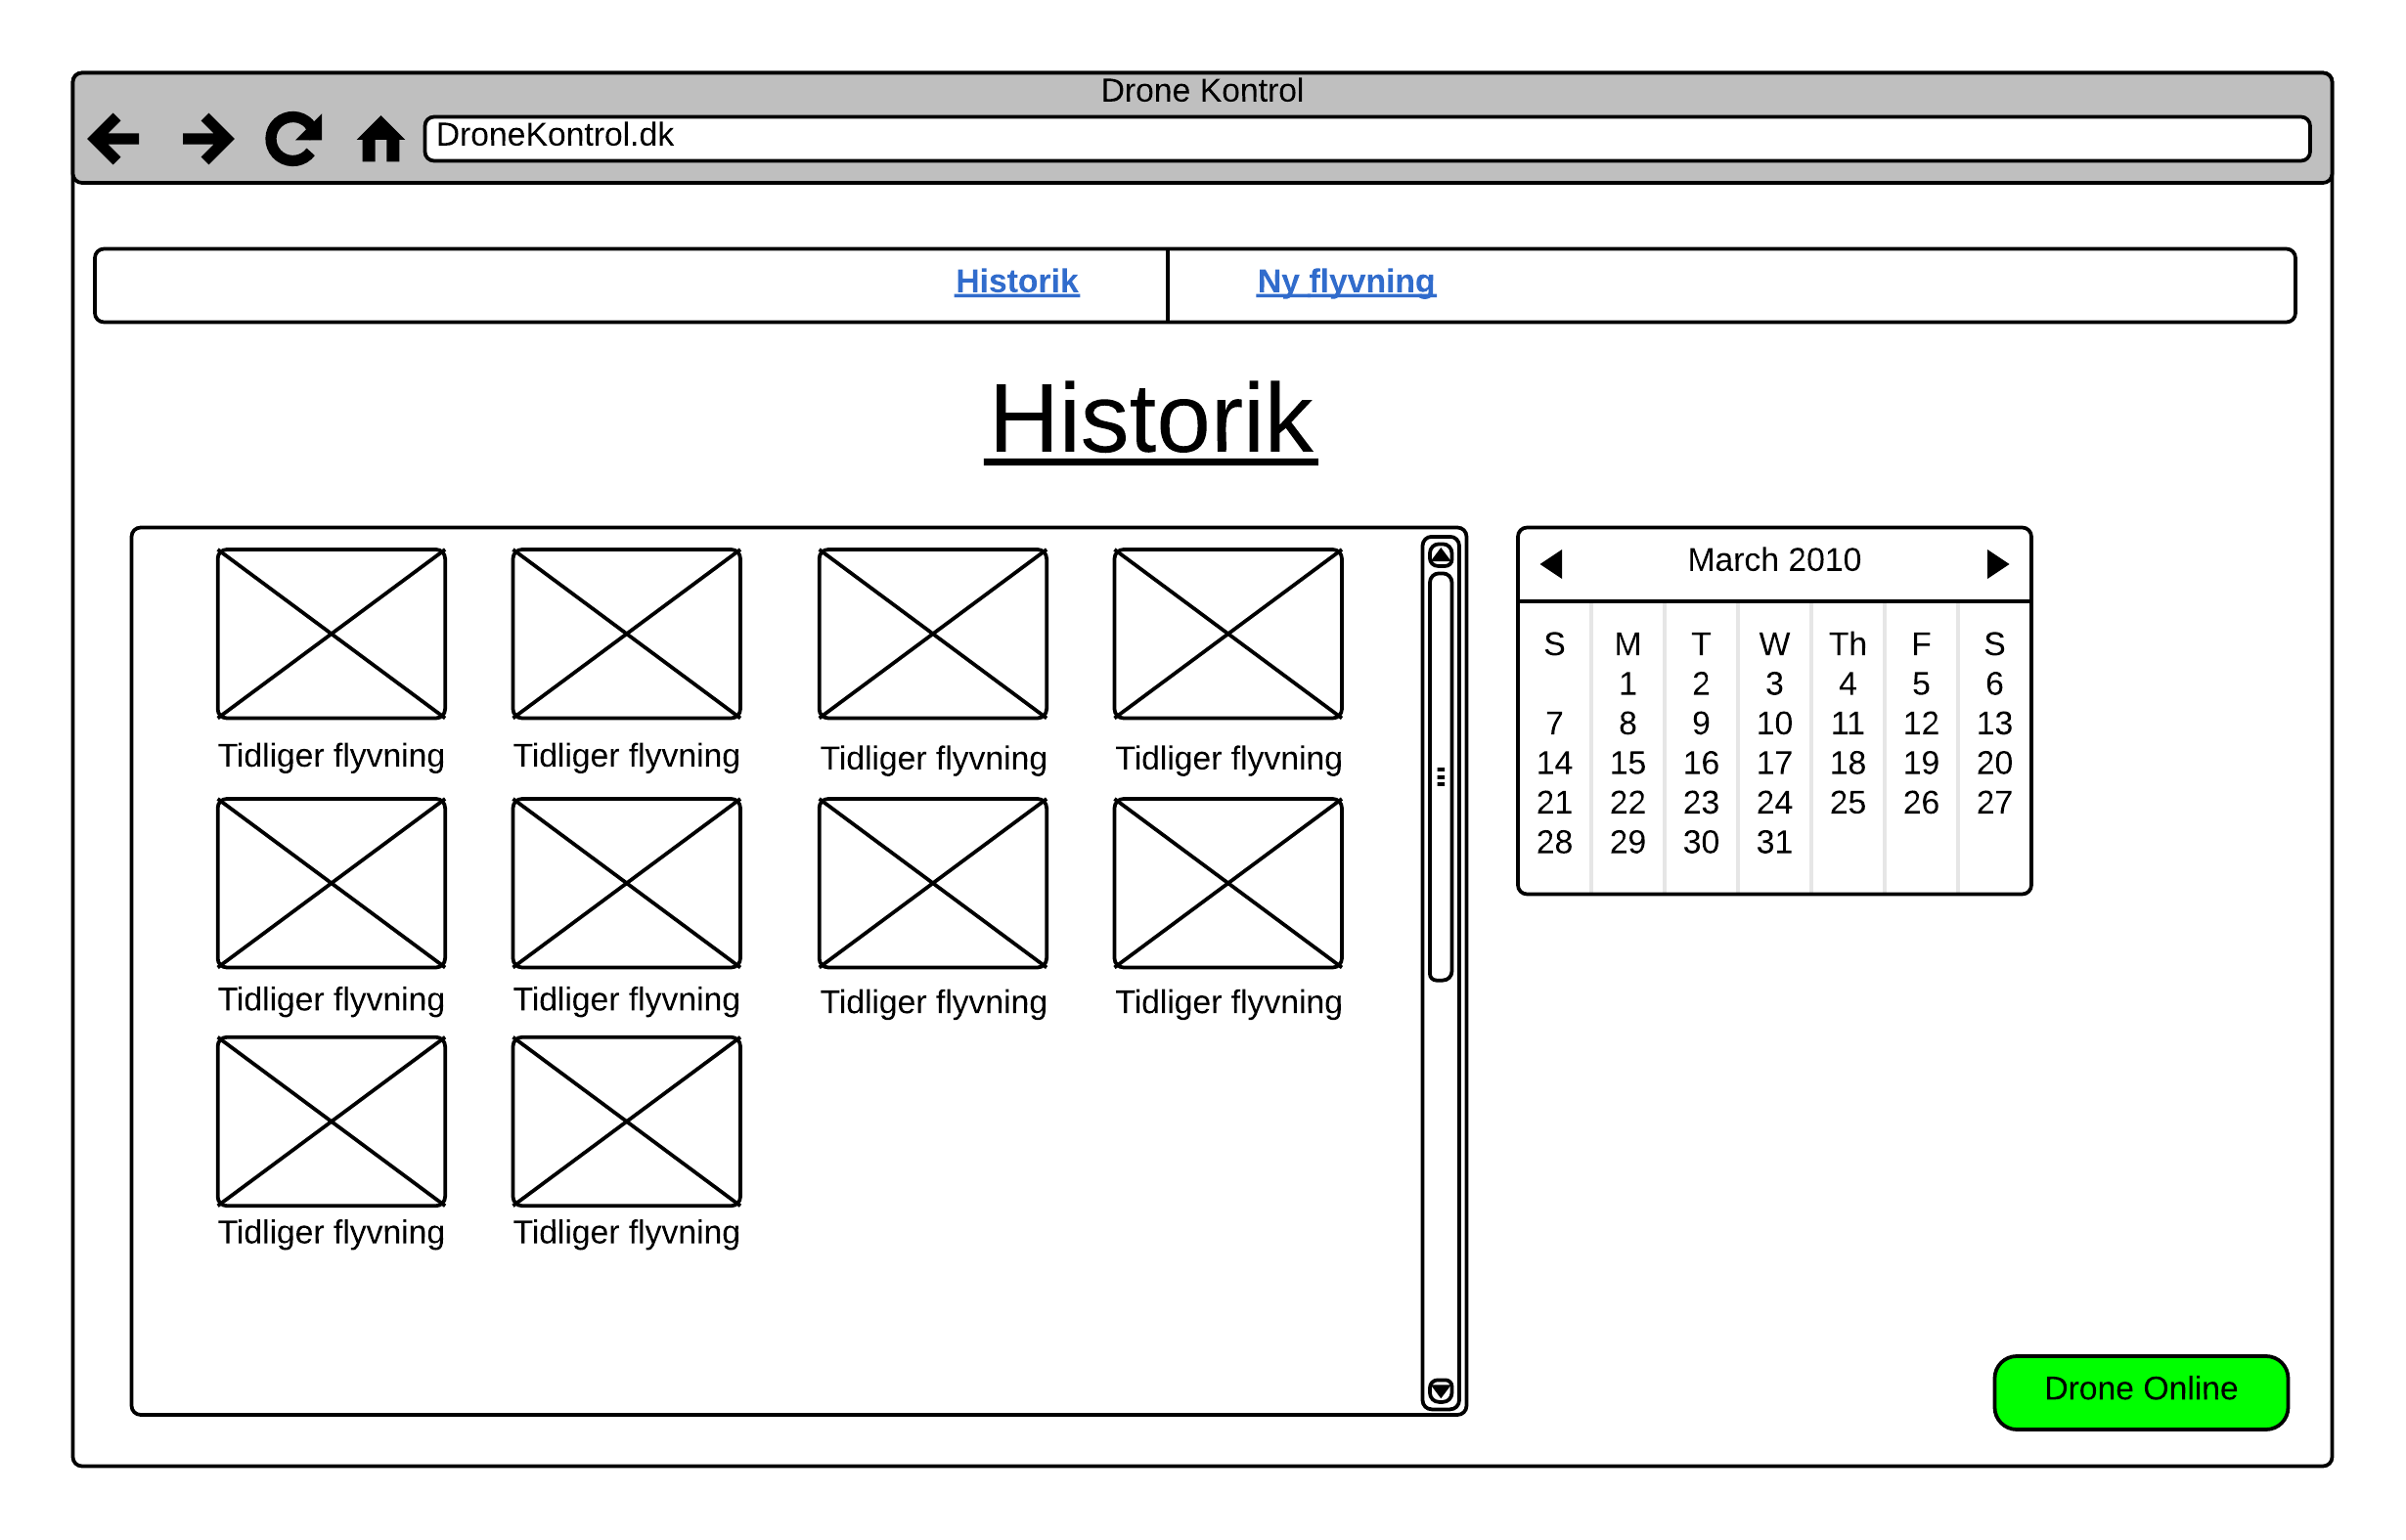
\includegraphics[width=0.9\textwidth]{Billeder/UI_mockups/archive.png}
	\vspace{-.5cm}
	\caption{Historik vindue}
	\label{fig:mockup_archive}
\end{figure}

\newpage

Når en tidligere flyvning er valgt, præsenteres bruger for al information tilknyttet den pågældende flyvning. Dette giver bruger adgang til flyveopsætninger og billeder. På et kort vises den flyveruten dronen gjorde brug af.

\vspace{-5pt}
%Archive choosen mockup
\begin{figure}[H]
	\centering
	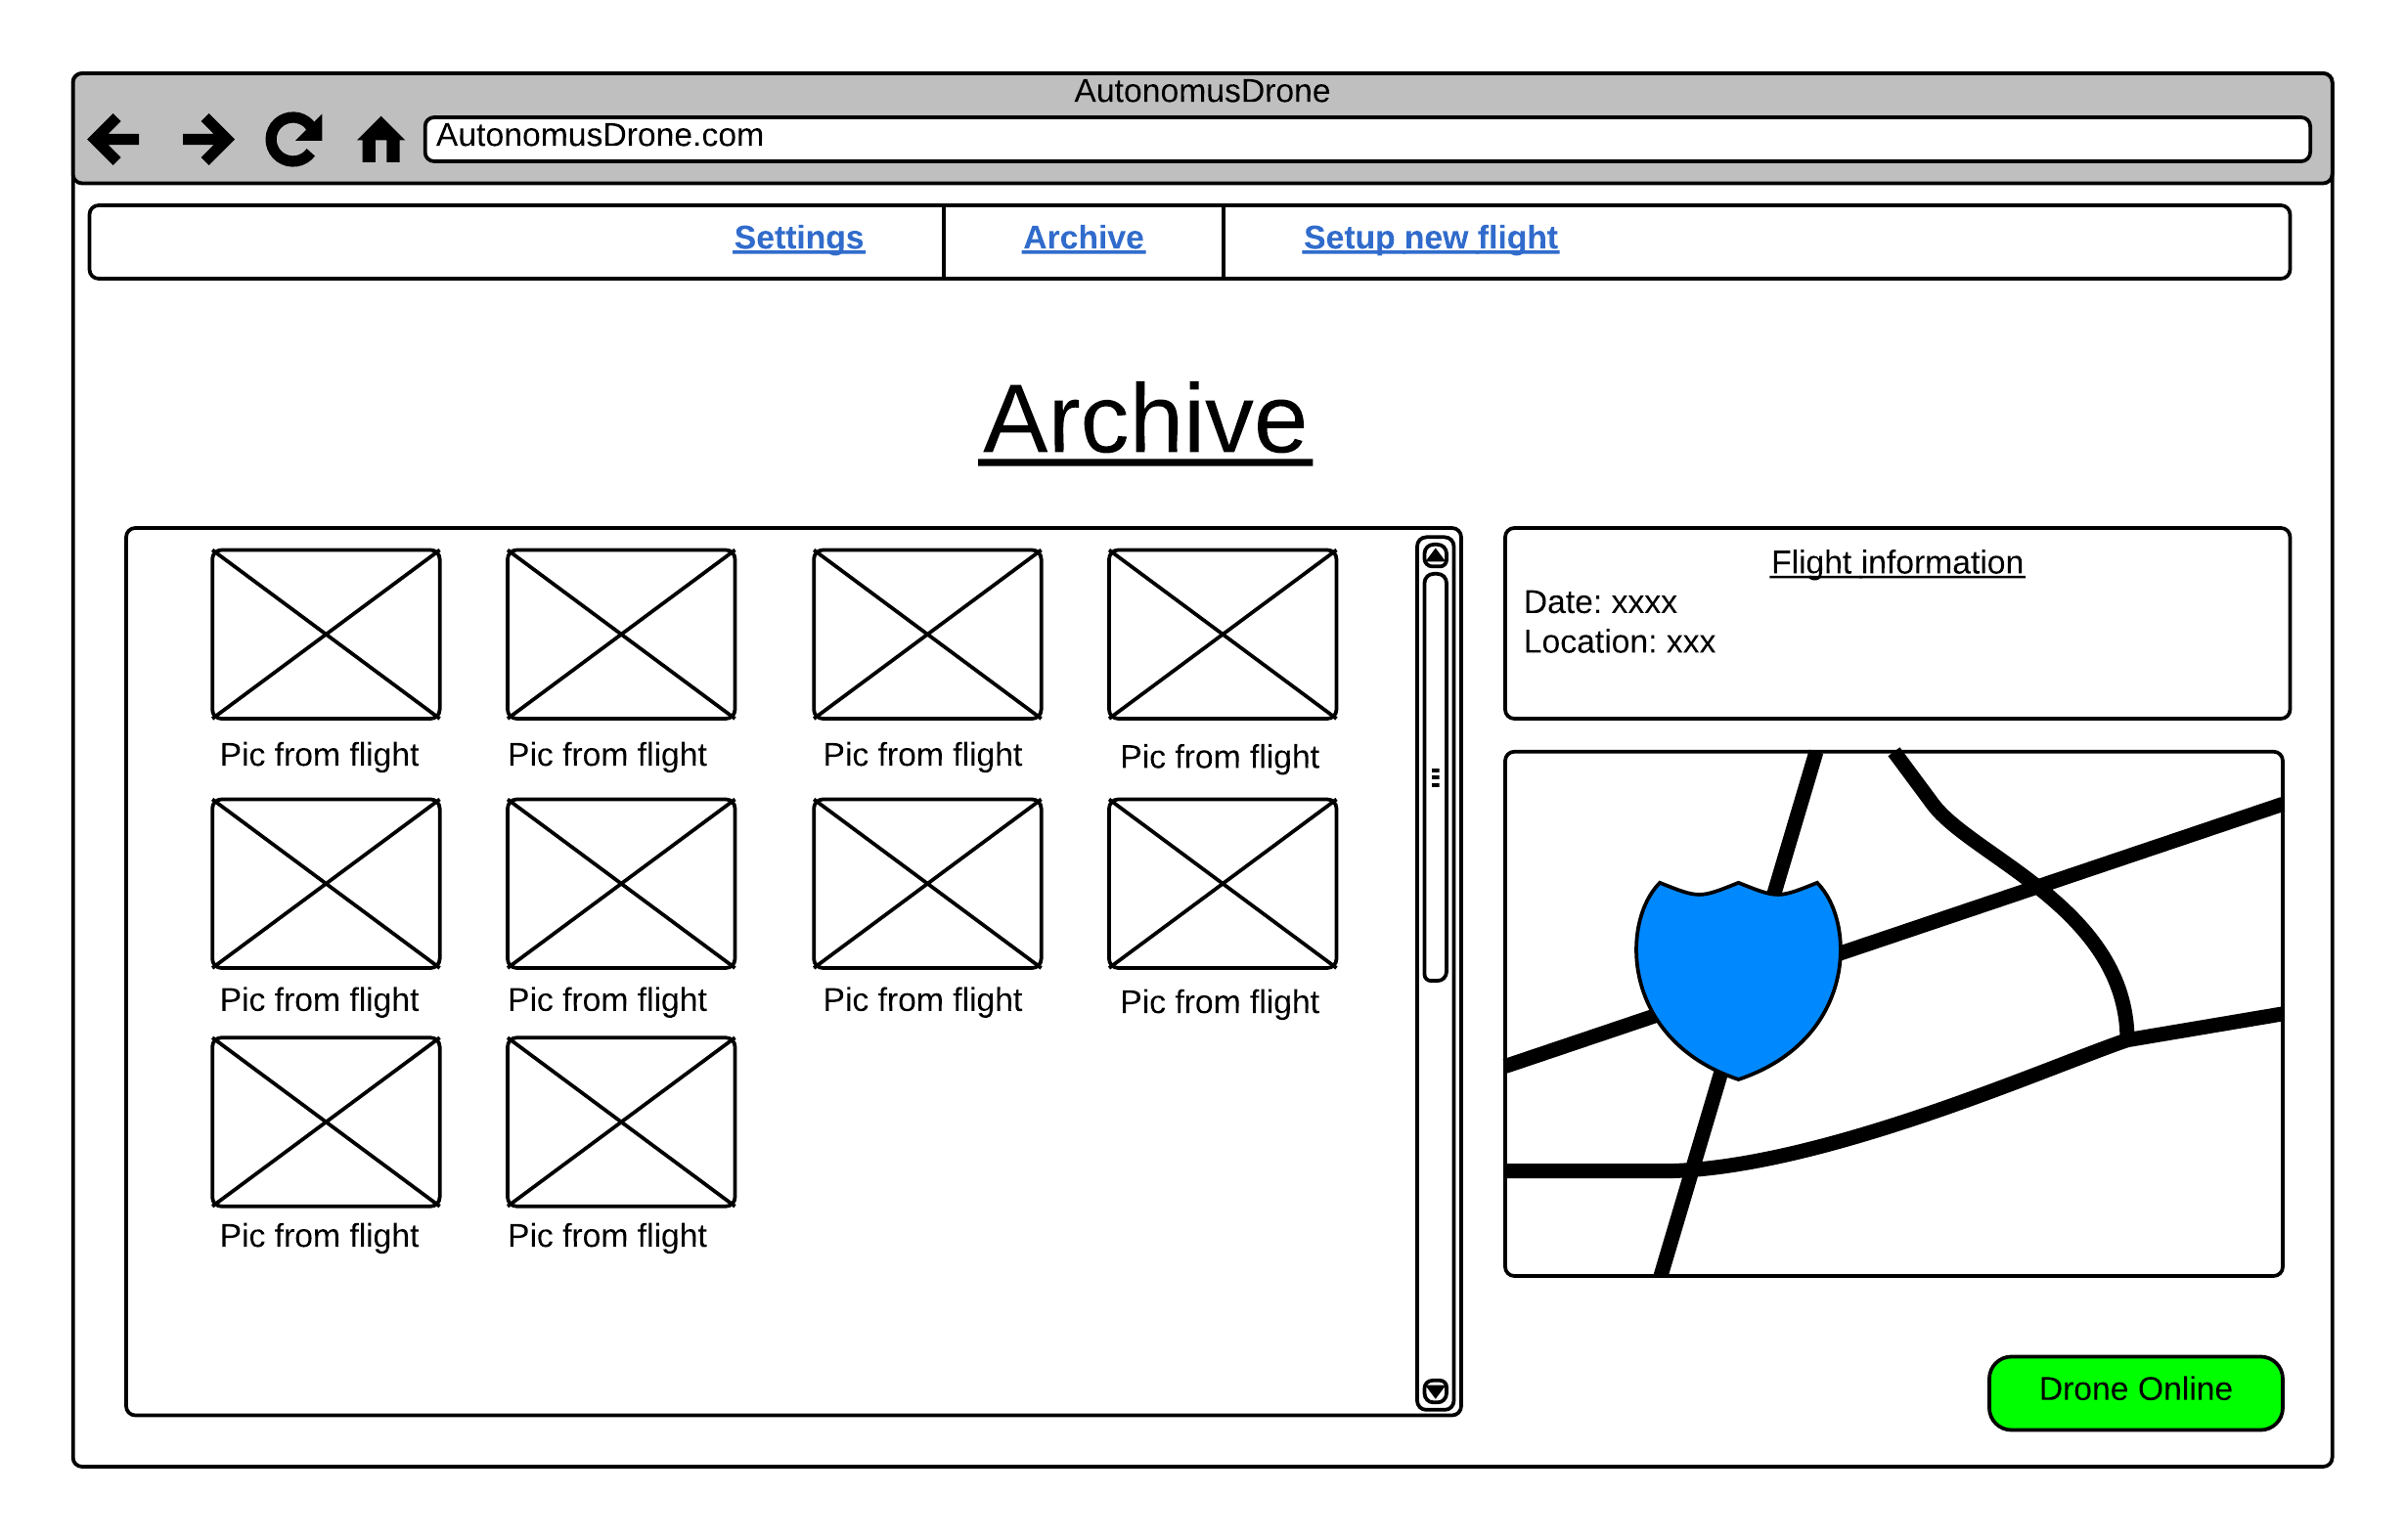
\includegraphics[width=0.9\textwidth]{Billeder/UI_mockups/archive_choosen.png}
	\vspace{-.5cm}
	\caption{Tidligere flyverute valgt}
	\label{fig:mockup_archive_choosen}
\end{figure}


I ny flyveopsætnings menuen kan bruger indstille nye flyveopsætninger. 
Bruger kan indstille sin ønskede flyverute ved at klikke på kortet, og vælge hvilke GPS positioner som dronen skal overvåge og tage billeder af. 
Hver GPS position der vælges præsenteres i tabellen til venstre for kortet. 
I tabellen kan bruger ydermere indstille om der skal tages billeder ved GPS positionerne og hvilken højde dronen skal tage billeder fra. Nedenfor tabellen sættes den generelle flyvehøjde.
Bruger har mulighed for at gemme nylavede flyveopsætninger til senere brug.

\vspace{-5pt}
%Setup new flight mockup
\begin{figure}[H]
	\centering
	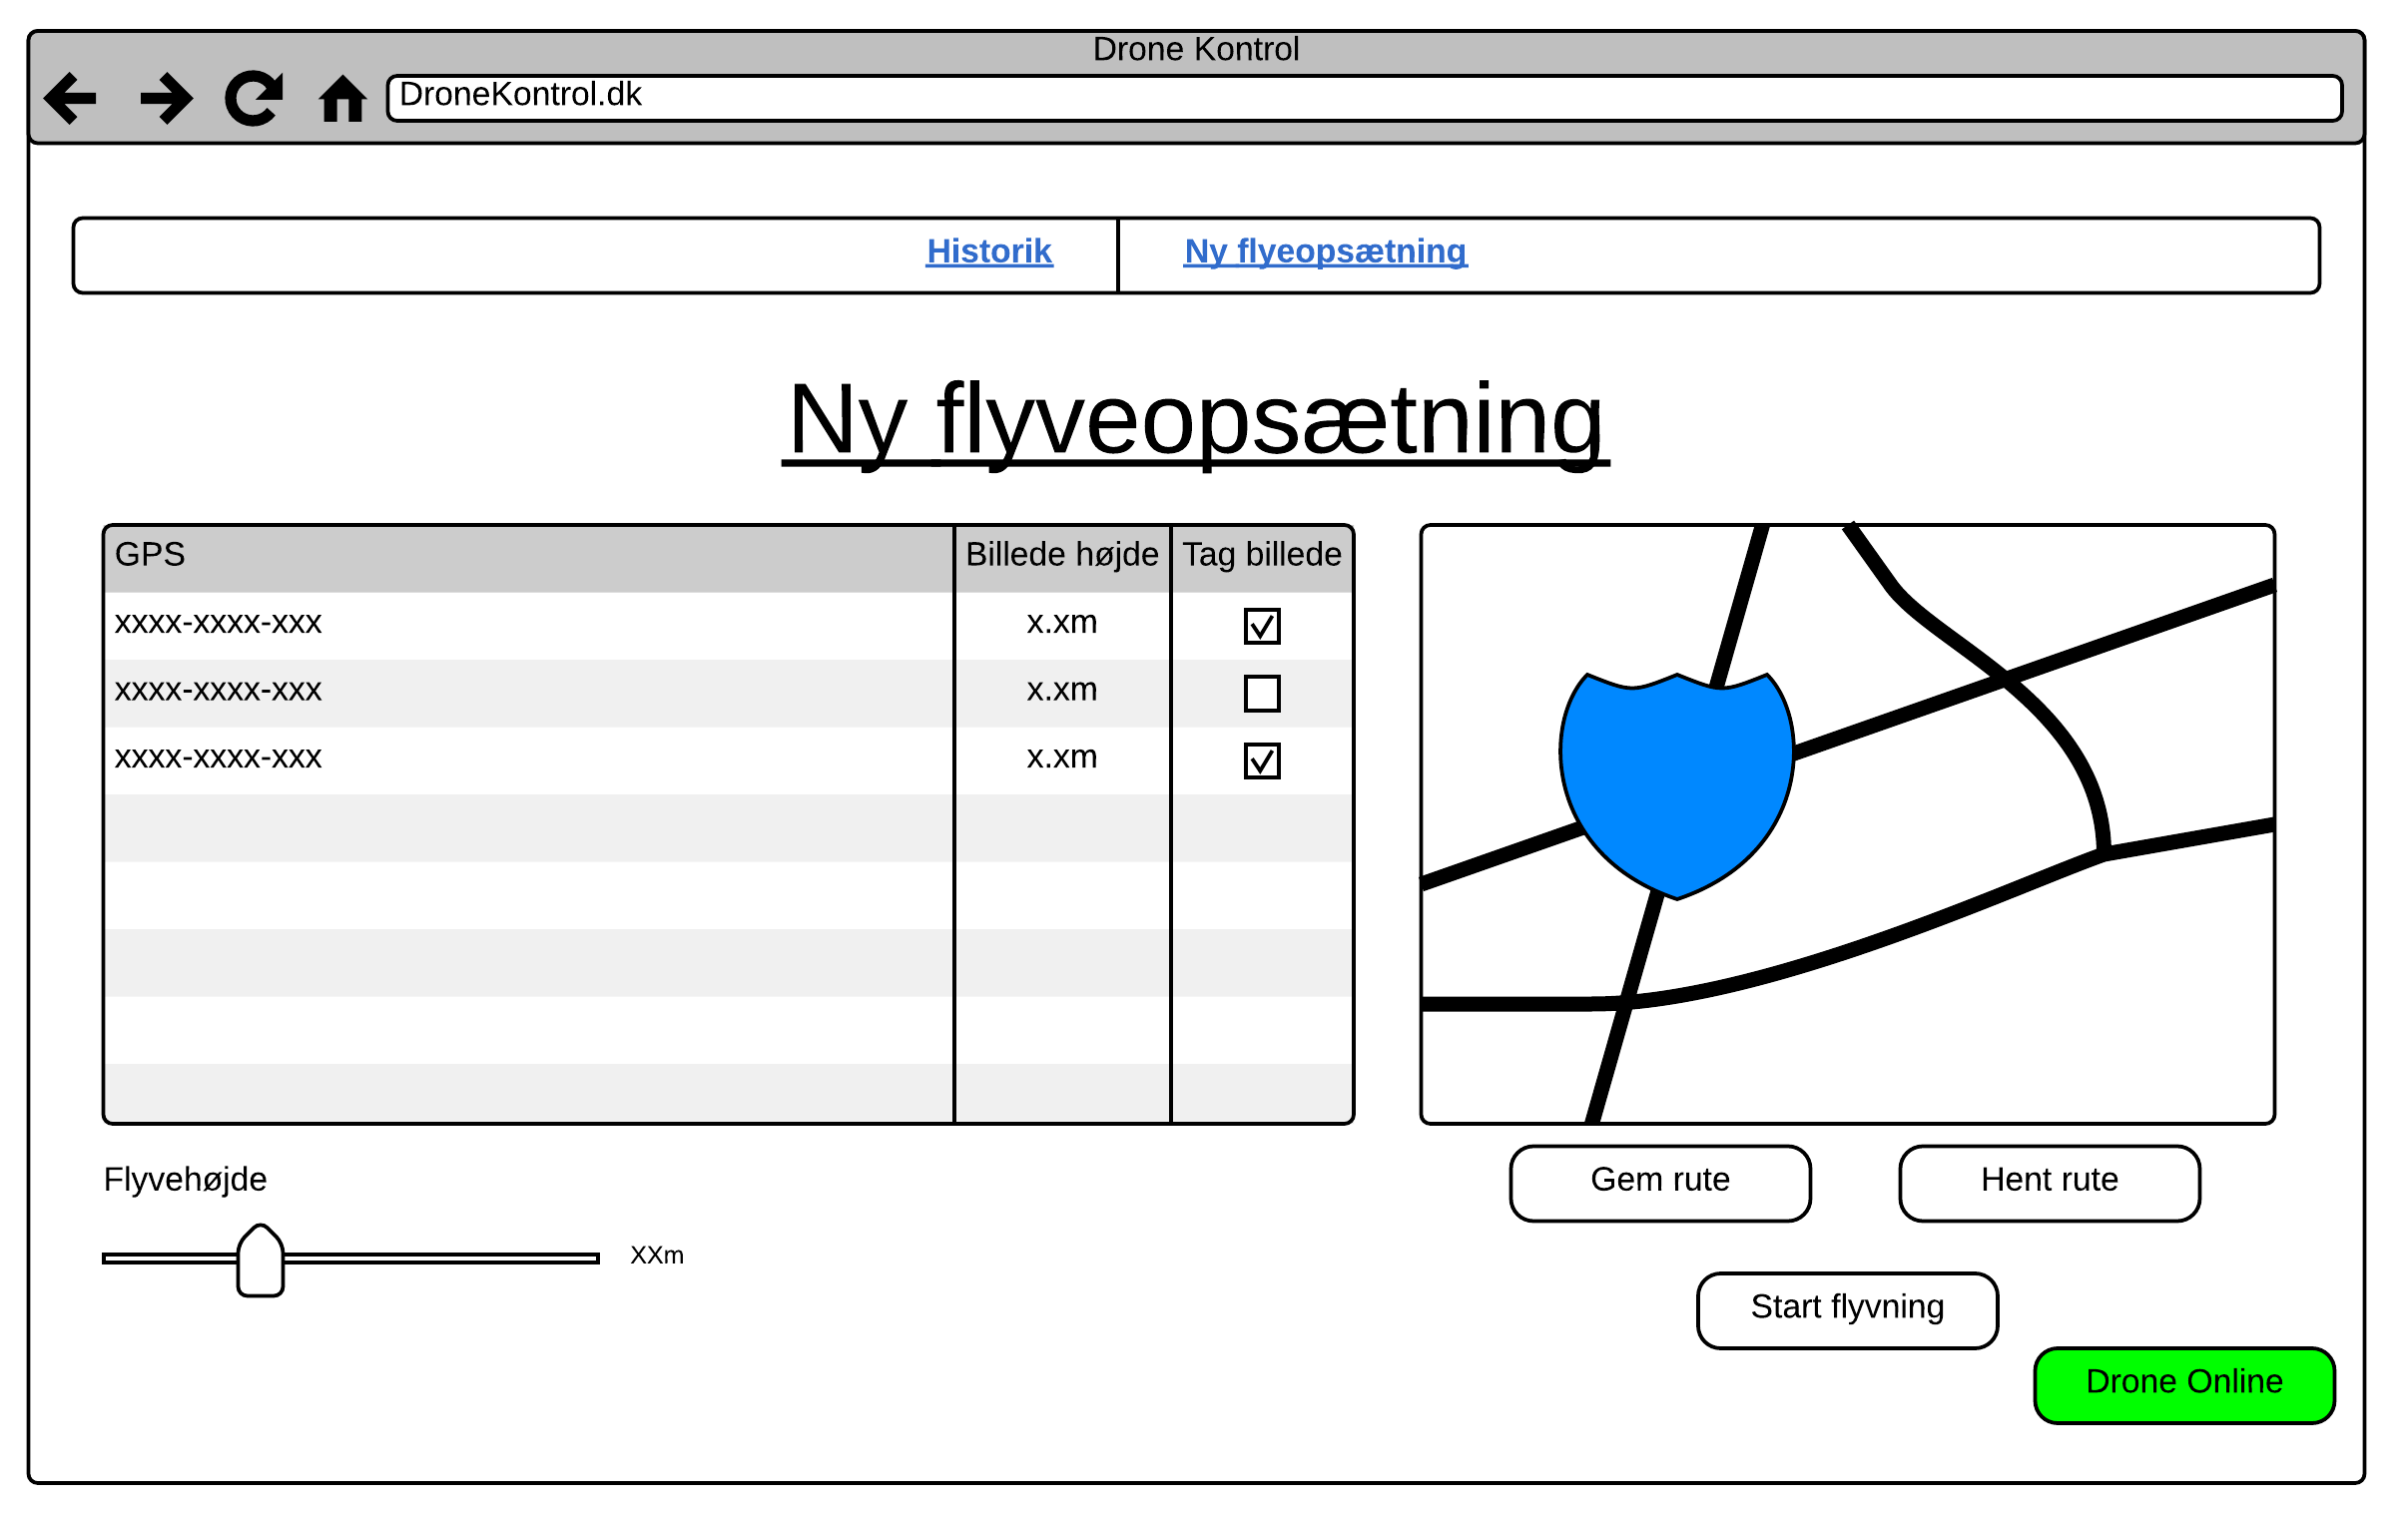
\includegraphics[width=0.9\textwidth]{Billeder/UI_mockups/setup_new_flight.png}
	\vspace{-.2cm}
	\caption{Ny flyverute}
	\label{fig:mockup_setup_new_flight}
\end{figure}

 